\documentclass[conference]{IEEEtran}

% --- Packages ---
\usepackage[utf8]{inputenc}
\usepackage{tikz}
\usetikzlibrary{arrows.meta, positioning, shapes.geometric}
\usepackage{pgfplots}
\pgfplotsset{compat=1.18}
\usepackage{hyperref}
\usepackage{array}
\usepackage{booktabs}
\usepackage{cite}
\usepackage{amsmath}
\usepackage[strings]{underscore} % makes _ safe in text
\usepackage{float} % for [H] placement if needed

% --- Title & Authors ---
\title{Clinical Data Extraction from Medical Reports using GBERT-based Named Entity Recognition}

\author{
    \IEEEauthorblockN{Michele Bufano}
    \IEEEauthorblockA{
        Department of Radiology,\\
        University Medical Center Freiburg, Germany\\
        Email: michele.bufano@uniklinik-freiburg.de
    }
}
\setlength{\textwidth}{6.5in}
\setlength{\emergencystretch}{2em}  % Allow LaTeX to stretch spaces to avoid overflow
\sloppy  % Make LaTeX more forgiving about line breaks
\begin{document}
\maketitle

% --- Abstract ---
\begin{abstract}
Clinical reports contain valuable patient data, yet most of this information is stored as unstructured text. Extracting structured entities is essential for clinical research, interoperability, and decision support. We present an open-source pipeline for Named Entity Recognition (NER) in German clinical texts, based on GBERT. The system integrates synthetic data generation, model fine-tuning, and a prediction pipeline capable of processing diverse input formats (PDF, DOCX, images, plain text). Preliminary results demonstrate promising extraction quality, with ongoing evaluation and interoperability integration planned.
\end{abstract}

\begin{IEEEkeywords}
Named Entity Recognition, GBERT, Clinical NLP, German, Electronic Health Records
\end{IEEEkeywords}

% --- Introduction ---
\section{Introduction}
Electronic Health Records (EHRs) store both structured fields and free-text documents. While structured fields are machine-readable, clinical knowledge is often embedded in narrative reports. This makes downstream applications---such as automated coding, patient cohort identification, or decision support---difficult.

Named Entity Recognition (NER) provides a way to extract structured concepts from text. In English, models such as BioBERT and ClinicalBERT have achieved state-of-the-art results, but resources for German remain limited. We address this by leveraging GBERT, a transformer-based model for German, and tailoring it to clinical NER.

% --- Methods ---
\section{Methods}

\subsection{Data}
Training requires token-level annotations in BIO format. Since large annotated German clinical datasets are scarce, we implemented a synthetic data generator using templates and paraphrases. This produces training, validation, and test sets in JSON format.

\subsection{Model}
We fine-tuned GBERT-base using the Hugging Face framework. The model receives full sentences as input and predicts token-level entity labels. Predicted tokens are merged into entity spans with type, text span, and confidence score.

\subsection{Pipelines}
The system consists of two main pipelines: training and prediction.  

\begin{figure}[htbp]
    \centering
    \resizebox{\linewidth}{!}{%
    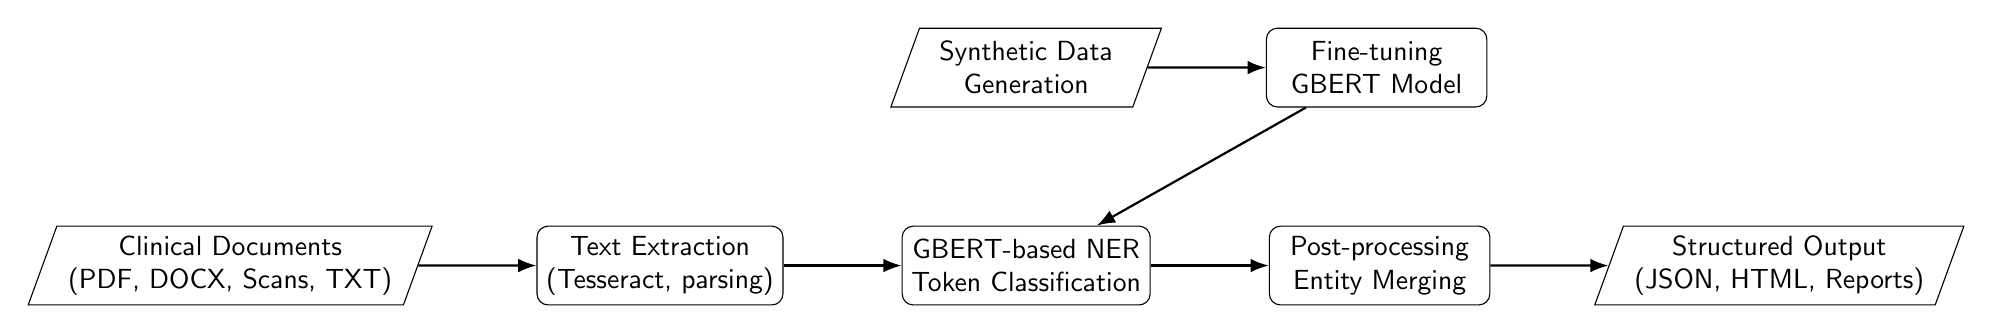
\begin{tikzpicture}[
        node distance=1.8cm and 1.5cm,
        every node/.style={font=\sffamily},
        process/.style={rectangle, draw, rounded corners, minimum width=2.8cm, minimum height=1cm, align=center},
        io/.style={trapezium, trapezium left angle=70, trapezium right angle=110, draw, minimum width=3cm, minimum height=1cm, align=center},
        arrow/.style={-Latex, thick}
    ]
        % Nodes
        \node[io] (input) {Clinical Documents\\ (PDF, DOCX, Scans, TXT)};
        \node[process, right=of input] (ocr) {Text Extraction\\ (Tesseract, parsing)};
        \node[process, right=of ocr] (model) {GBERT-based NER\\ Token Classification};
        \node[process, right=of model] (post) {Post-processing\\ Entity Merging};
        \node[io, right=of post] (output) {Structured Output\\ (JSON, HTML, Reports)};

        % Training pipeline on top
        \node[io, above=1.5cm of model] (synthetic) {Synthetic Data\\ Generation};
        \node[process, right=of synthetic] (training) {Fine-tuning\\ GBERT Model};

        % Arrows (Prediction)
        \draw[arrow] (input) -- (ocr);
        \draw[arrow] (ocr) -- (model);
        \draw[arrow] (model) -- (post);
        \draw[arrow] (post) -- (output);

        % Arrows (Training)
        \draw[arrow] (synthetic) -- (training);
        \draw[arrow] (training) -- (model);

    \end{tikzpicture}%
    }
    \caption{System architecture: training pipeline (top) and prediction pipeline (bottom).}
    \label{fig:pipeline}
\end{figure}

\section{Evaluation and Validation}
Model validation is a crucial step to assess the quality of extracted entities. 
Our framework supports an end-to-end evaluation workflow based on synthetic data generation and prediction comparison.

\subsection{Synthetic Reference Data}
Each generated synthetic sample is produced in two formats:
\begin{itemize}
    \item \textbf{NER JSON}: {\raggedright token-level annotations in BIO scheme, serving as ground truth.\par}
    \item \textbf{Text report}: a plain-text clinical note created from the same template, which can be processed by the prediction pipeline.
\end{itemize}

\subsection{Prediction and Comparison}
The prediction pipeline processes the text reports and produces structured entity outputs in JSON. 
These predictions are then compared against the ground truth NER JSON. 
The comparison script aligns predicted entity spans with reference spans and computes standard metrics:
\begin{itemize}
    \item \textbf{Precision}: proportion of correctly predicted entities among all predicted entities.
    \item \textbf{Recall}: proportion of correctly predicted entities among all reference entities.
    \item \textbf{F1-score}: harmonic mean of precision and recall.
\end{itemize}
\begin{figure}[htbp]
    \centering
    \resizebox{\linewidth}{!}{%
    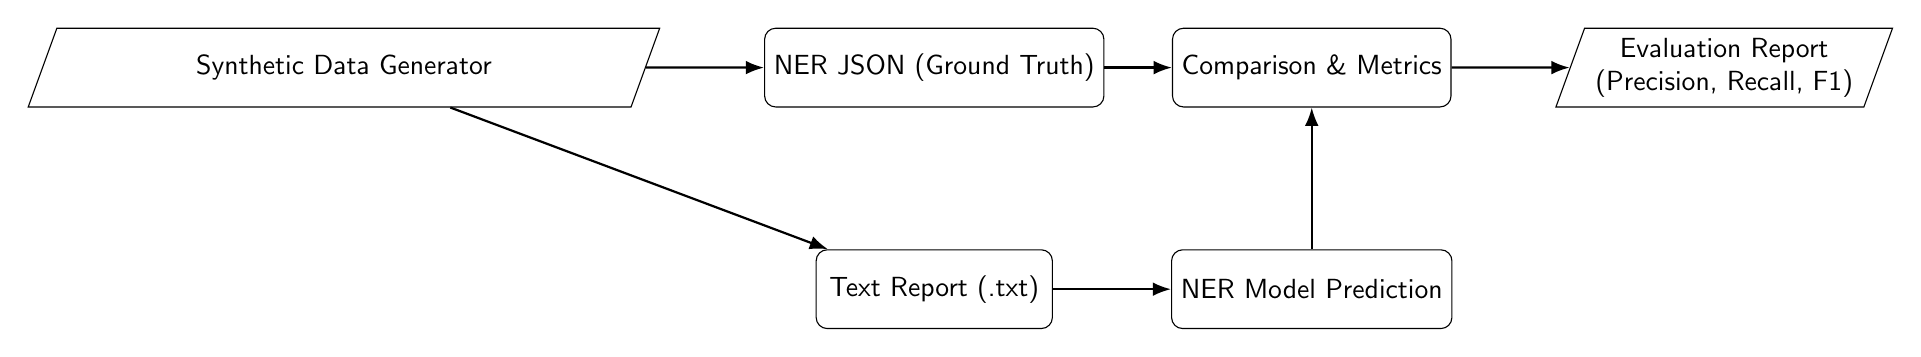
\begin{tikzpicture}[
        node distance=1.8cm and 1.5cm,
        every node/.style={font=\sffamily},
        process/.style={rectangle, draw, rounded corners, minimum width=3cm, minimum height=1cm, align=center},
        io/.style={trapezium, trapezium left angle=70, trapezium right angle=110, draw, minimum width=3.2cm, minimum height=1cm, align=center},
        arrow/.style={-Latex, thick}
    ]
        % Nodes
        \node[io] (synthetic) {Synthetic Data Generator};
        \node[process, right=of synthetic] (groundtruth) {NER JSON (Ground Truth)};
        \node[process, below=of groundtruth] (txt) {Text Report (.txt)};
        \node[process, right=of txt] (prediction) {NER Model Prediction};
        \node[process, above=of prediction] (compare) {Comparison \& Metrics};
        \node[io, right=of compare] (report) {Evaluation Report\\ (Precision, Recall, F1)};

        % Arrows
        \draw[arrow] (synthetic) -- (groundtruth);
        \draw[arrow] (synthetic) -- (txt);
        \draw[arrow] (txt) -- (prediction);
        \draw[arrow] (groundtruth) -- (compare);
        \draw[arrow] (prediction) -- (compare);
        \draw[arrow] (compare) -- (report);
    \end{tikzpicture}
    }
    \caption{Validation workflow: synthetic data is generated in both annotated JSON and plain-text format. The text report is processed by the model, predictions are compared against the ground truth JSON, and metrics are computed.}
    \label{fig:validation}
\end{figure}


\subsection{Evaluation Reports}
{\raggedright For each validation run, the system outputs an \texttt{evaluation\_report.json} including: \par}
\begin{itemize}
    \item Entity-level results (true positives, false positives, false negatives).
    \item Global metrics per label type (e.g., ORG, DATE, DIAGNOSIS).
    \item Confusion analysis highlighting frequent misclassifications.
\end{itemize}

This design allows rapid testing of new model versions against a reproducible synthetic benchmark. 
Future work will extend the validation to annotated real-world datasets for more representative performance estimates.








\section{Evaluation}
Evaluation is performed by comparing predictions against reference annotations using precision, recall, and F1-score. A validation script reports detected spans and labels. Current experiments focus on synthetic data and small real-world samples; larger gold-standard datasets are planned.
Figure~\ref{fig:evaluation} shows precision, recall, and F1-scores for selected entity types (see end of document).

\begin{table}[htbp]
\centering
\caption{Example entity extraction output (synthetic report).}
\begin{tabular}{@{}p{2cm}p{2cm}p{2cm}@{}}
\toprule
\textbf{Token} & \textbf{Gold Label} & \textbf{Predicted Label} \\ \midrule
Microsoft      & B-ORG               & B-ORG \\
Inc.           & I-ORG               & I-ORG \\
April 4, 1975  & B-DATE              & B-DATE \\
Bill Gates     & B-PER               & B-PER \\
Albuquerque    & B-LOC               & B-LOC \\ \bottomrule
\end{tabular}
\label{tab:example}
\end{table}


% --- Results ---
\section{Results}
Initial experiments on synthetic reports show that the validation pipeline 
(Figure~\ref{fig:validation}) can reliably compare predictions against reference annotations. 
High precision and recall are obtained for well-structured entities such as \texttt{DATE} and \texttt{ORG}, 
while performance on more complex clinical terms (e.g., \texttt{DIAGNOSIS}, \texttt{MEDICATION}) remains more challenging.

Table~\ref{tab:example} illustrates an example of token-level alignment between 
gold-standard labels and predicted labels. Figure~\ref{fig:evaluation} summarizes 
aggregated performance across selected entity types.

These results confirm that the system is suitable for structured entities with 
unambiguous boundaries, and provide a reproducible baseline for model 
improvements in future iterations.

% --- Discussion & Future Work ---
\section{Discussion and Future Work}
This work demonstrates that GBERT-based NER can extract structured information from German clinical texts, even when trained with synthetic data. Challenges remain:
\begin{itemize}
    \item Limited availability of annotated German clinical corpora.
    \item Entity boundary ambiguity in free-text notes.
    \item Need for robust evaluation on real-world datasets.
\end{itemize}

Future work includes:
\begin{itemize}
    \item \textbf{FHIR integration:} Planned mappings of NER labels to HL7 FHIR resources are summarized in Table~\ref{tab:fhir}.
    \item \textbf{DICOM Structured Report (SR):} Embedding extracted entities into DICOM SR objects, enabling integration into imaging workflows.
    \item \textbf{Expanded evaluation:} {\raggedright Benchmarking on real-world annotated datasets.\par}
    \item \textbf{Domain-specific vocabularies:} {\raggedright Adapting the model with clinical ontologies and terminologies.\par}
\end{itemize}

\subsection{Use Case Scenario}
To illustrate the clinical utility, consider the following simplified medical note:

\begin{quote}

{\raggedright ``Herr Müller wurde am 12.03.2024 mit Brustschmerzen in die Kardiologie des Universitätsklinikums aufgenommen. Der behandelnde Arzt Dr. Schmidt diagnostizierte einen Myokardinfarkt und verordnete Aspirin.'' \par}
\end{quote}

Our NER system would extract:
\begin{itemize}
    \item \textbf{PERSON:} Herr Müller
    \item \textbf{DATE:} 12.03.2024
    \item \textbf{SYMPTOM:} Brustschmerzen
    \item \textbf{DEPARTMENT:} Kardiologie
    \item \textbf{ORGANIZATION:} Universitätsklinikum
    \item \textbf{DOCTOR:} Dr. Schmidt
    \item \textbf{DIAGNOSIS:} Myokardinfarkt
    \item \textbf{MEDICATION:} Aspirin
\end{itemize}

These entities could be mapped into structured FHIR resources:

\begin{itemize}
    \item A \texttt{Patient} resource for Herr Müller.
    \item A \texttt{Practitioner} resource for Dr. Schmidt.
    \item A \texttt{Condition} resource for Myokardinfarkt with onset date 12.03.2024.
    \item {\raggedright An \texttt{Observation} resource for the symptom Brustschmerzen. \par}
    \item A \texttt{MedicationRequest} resource for Aspirin.
    \item An \texttt{Encounter} resource linking the patient to the Universitätsklinikum and the cardiology department.
\end{itemize}

% --- Conclusion ---
\section{Conclusion}
We introduce a GBERT-based NER system for German clinical texts, including data generation, training, and prediction pipelines. The open-source implementation supports heterogeneous document formats and lays the foundation for future interoperable clinical NLP applications.

% --- Availability ---
\section*{Availability}

{\raggedright Code and documentation: \href{https://github.com/rtdicomexplorer/medical_ner_classification}{https://github.com/rtdicomexplorer/medical_ner_classification} \par}

% --- References ---
\bibliographystyle{IEEEtran}
\begin{thebibliography}{99}

\bibitem{bert}
Devlin, J., Chang, M.-W., Lee, K., \& Toutanova, K. (2019). BERT: Pre-training of Deep Bidirectional Transformers for Language Understanding. \textit{NAACL}.

\bibitem{transformers}
Wolf, T., Debut, L., Sanh, V., et al. (2020). Transformers: State-of-the-Art NLP Library. \textit{EMNLP}.

\bibitem{fhir}
HL7 International. (2023). FHIR Standard. \url{https://hl7.org/fhir}.

\end{thebibliography}

\onecolumn

\begin{figure}[htbp]
    \centering
    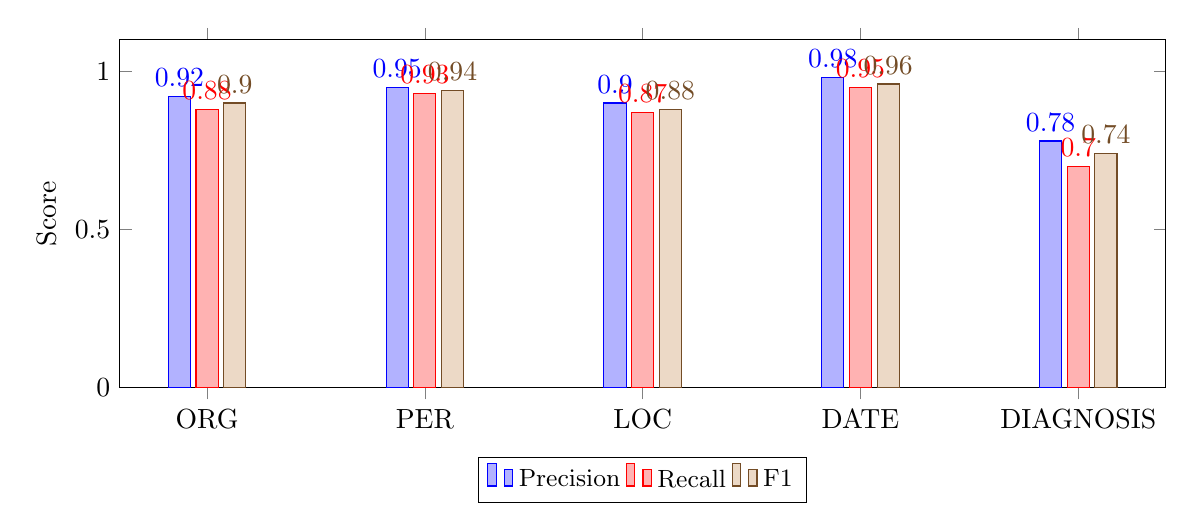
\begin{tikzpicture}
        \begin{axis}[
            ybar,
            bar width=8pt,
            width=0.9\linewidth,
            height=6cm,
            ymin=0, ymax=1.1,
            ylabel={Score},
            symbolic x coords={ORG, PER, LOC, DATE, DIAGNOSIS},
            xtick=data,
            nodes near coords,
            nodes near coords align={vertical},
            legend style={font=\small,at={(0.5,-0.2)},anchor=north,legend columns=-1},
            ylabel near ticks
        ]
        \addplot coordinates {(ORG,0.92) (PER,0.95) (LOC,0.90) (DATE,0.98) (DIAGNOSIS,0.78)};
        \addplot coordinates {(ORG,0.88) (PER,0.93) (LOC,0.87) (DATE,0.95) (DIAGNOSIS,0.70)};
        \addplot coordinates {(ORG,0.90) (PER,0.94) (LOC,0.88) (DATE,0.96) (DIAGNOSIS,0.74)};
        \legend{Precision, Recall, F1}
        \end{axis}
    \end{tikzpicture}
    \caption{Evaluation results (dummy values ). Precision, recall, and F1-score across selected entity types.}
    \label{fig:evaluation}
\end{figure}


\begin{table}[htbp]
\centering
\caption{Planned mapping of NER labels to HL7 FHIR resources (future work).}
\begin{tabular}{@{}p{3cm}p{5cm}p{5cm}@{}}  % adjust column widths for full page
\toprule
\textbf{NER Label} & \textbf{Example Entities} & \textbf{FHIR Resource} \\
\midrule
PERSON          & Patient, Family member        & Patient, RelatedPerson \\
DOCTOR          & Physician, Specialist         & Practitioner \\
ORGANIZATION    & Hospital, Clinic              & Organization \\
DATE            & Admission date, DOB           & Date fields \\
DIAGNOSIS       & Disease names                 & Condition \\
SYMPTOM         & Clinical findings             & Observation \\
MEDICATION      & Drugs, prescriptions          & MedicationRequest \\
PROCEDURE       & Surgeries, exams              & Procedure \\
TREATMENT       & Therapies, care plans         & CarePlan, Procedure \\
DEPARTMENT      & Hospital units                & Location, Organization \\
LAB\_RESULT     & Blood test values             & Observation \\
ALLERGY         & Allergies                     & AllergyIntolerance \\
IMMUNIZATION    & Vaccines                      & Immunization \\
DEVICE          & Medical devices               & Device \\
FAMILY\_HISTORY & Family medical history        & FamilyMemberHistory \\
\bottomrule
\end{tabular}
\label{tab:fhir}
\end{table}
\twocolumn




\end{document}

